\documentclass[12pt]{article}

\usepackage{pablo}
\usepackage{pablo-listings}
\usepackage{multicol}
\usepackage[a5paper,margin=2cm]{geometry}
\usepackage{tkz-tab}
\pagestyle{empty}

\begin{document}

\begin{center}
\textsc{Devoir}

Corrigé
\end{center}
\hrule

\begin{exercice}[Probabilités --- 5 points]
  On considère un jeu de 32 cartes.
  \begin{enumerate}
    \item \emph{On tire une carte au hasard. Quelle est la probabilité de tirer un As ?} Il y a équiprobabilités, et quatre As dans un jeu de 32 cartes, donc la probabilité est $\frac{4}{32}=\frac{1}{8}$.
    \item \emph{On tire deux cartes au hasard, sans remise, et on s'intéresse aux As tirés.}
    \begin{enumerate}
      \item \emph{Représenter cette expérience par un arbre.}
      \item \emph{Quelle est la probabilité de tirer deux As ?} Une seule branche de l'arbre correspond à cet évènement. Sa probabilité est
        $\frac{4}{32}\times\frac{3}{31}=\frac{3}{248}\approx1,2\%$.
      \item \emph{Quelle est la probabilité de tirer exactement un As ?} Deux branches correspondent à cet évènement. Sa probabilité est donc la somme de ces deux branches, soit
        $\frac{4}{32}\times\frac{28}{31}+
        \frac{28}{32}\times\frac{4}{31}=\frac{7}{31}\approx23\%$.
    \end{enumerate}
  \end{enumerate}
  \begin{center}
    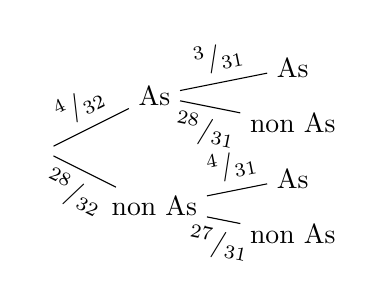
\begin{tikzpicture}[grow=right, sloped]
      % Set the overall layout of the tree
      \tikzstyle{level 1}=[level distance=4em, sibling distance=4em]
      \tikzstyle{level 2}=[level distance=5em, sibling distance=2em]
      \node {}
      child {
        node {non As}
        child {
          node {non As}
          edge from parent
          node[midway, below]{$^{27}/_{31}$}
        }
        child {
          node {As}
          edge from parent
          node[midway, above]{$^{4}/_{31}$}
        }
        edge from parent
        node[midway, below]{$^{28}/_{32}$}
      }
      child {
        node {As}
        child {
          node {non As}
          edge from parent
          node[midway, below]{$^{28}/_{31}$}
        }
        child {
          node {As}
          edge from parent
          node[midway, above]{$^{3}/_{31}$}
        }
        edge from parent
          node[midway, above]{$^{4}/_{32}$}
      };
    \end{tikzpicture}
  \end{center}
\end{exercice}

\begin{exercice}[Échantillonnage --- 6 points]~

  \emph{Travaillant dans un laboratoire de contrôle pharmaceutique, vous êtes chargé(e) d'étudier deux traitements $A$ et $B$, censés guérir une certaine maladie, pour autoriser ou non leur vente. On sait que 30\% des malades guérissent spontanément (c'est-à-dire sans médicament) en moins d'une semaine. La question à laquelle vous devez répondre est : Ces médicaments permettent-ils une guérison plus rapide ?}

  \begin{enumerate}
    \item \emph{Testé auprès de 30 personnes, le traitement $A$ en a guéri 17 en moins d'une semaine. On note $p_A$ la proportion théorique de malades guérissant en moins d'une semaine avec le médicament $A$.}
    \begin{enumerate}
      \item \emph{Déterminer un intervalle de confiance à 95~\% de $p_A$, donné par la formule $\left[f-\frac{1}{\sqrt{n}};f+\frac{1}{\sqrt{n}}\right]$, où $f$ est la fréquence des guérisons de l'échantillon en moins d'une semaine, et $n$ la taille de l'échantillon.} Le test a été mené sur 30 personnes, donc $n=30$, et 17 de ces personnes ont guéri en moins d'une semaine, donc $f=\frac{17}{30}$. Donc l'intervalle est $\left[\frac{17}{30}-\frac{1}{\sqrt{30}};\frac{17}{30}+\frac{1}{\sqrt{30}}\right]$, soit $[0,38;0,75]$.
      \item \emph{Pouvez-vous affirmer que ce médicament accélère le temps de guérison ? Justifier.} On peut affirmer, avec une probabilité d'erreur de 5\%, que la probabilité $p_A$ de guérison en moins d'une semaine avec ce médicament, est comprise dans l'intervalle $[0,38;0,75]$. Donc on peut affirmer, avec ce même taux d'erreur, que ce médicament accélère la vitesse de guérison.
    \end{enumerate}
    \item \emph{Un intervalle de confiance à 95~\% de la proportion $p_B$ de guérisons en moins d'une semaine avec le traitement $B$ est $\left[0,27;0,41\right]$. Pouvez-vous affirmer que ce traitement accélère la guérison ?} La proportion 30\% est comprise dans l'intervalle de confiance. Donc on ne peut affirmer, ni que ce médicament accélère la guérison, ni qu'il la ralentit.
    \item \emph{Parmi ces deux médicaments, le(s)quel(s) autoriseriez-vous à la vente ?} Nous autoriserions le premier médicament seulement, puisqu'il n'a pas été démontré que le second médicament accélère le temps de guérison.
  \end{enumerate}
\end{exercice}

\begin{exercice}[Tableau de signes --- 3 points]
  \emph{Résoudre l'inéquation suivante en utilisant un tableau de signes.}

  \[\frac{2x-3}{5-x}<0\]

  On commence par résoudre séparément chacune des deux inéquations $2x-3\geq0$ et $5-x\geq0$. Nous obtenons : $2x-3\geq0$ si et seulement si $x\geq\frac{3}{2}$, et $5-x\geq0$ si et seulement si $x\leq5$.

  \begin{center}
    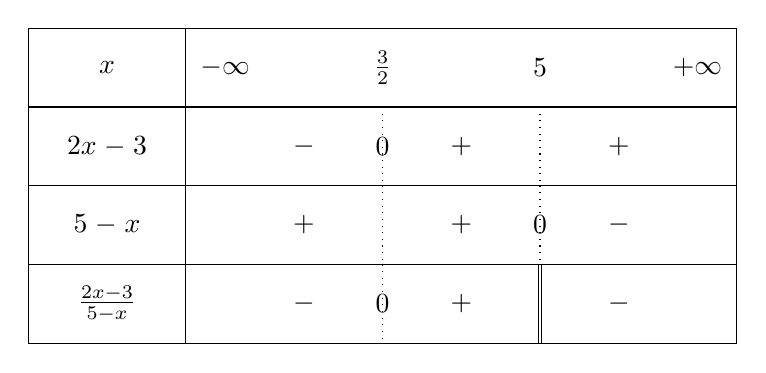
\begin{tikzpicture}
      \tkzTabInit[espcl=2]{$x$ /1, $2x-3$ /1, $5-x$ /1, $\frac{2x-3}{5-x}$/1 }%
      {$-\infty$ ,$\frac{3}{2}$ , $5$, $+\infty$}%
      \tkzTabLine{,-,z,+,t,+}
      \tkzTabLine{,+,t,+,z,-}
      \tkzTabLine{,-,z,+,d,-}
    \end{tikzpicture}
  \end{center}
  Les solutions sont donc $]-\infty;\frac{3}{2}[\cup]5;+\infty[$.
\end{exercice}

\begin{exercice}[Algorithmique --- 6 points]~

  On considère l'algorithme suivant.
  \begin{lstlisting}[language=naturel,frame=lines,mathescape=true]
  Lire x
  Si (2x-7)/(3-x) > 0
  Alors
  Afficher "Vrai"
  Sinon
  Afficher "Faux"
  FinSi
  \end{lstlisting}
  \begin{enumerate}
    \item \emph{Faire fonctionner cet algorithme avec $x=0$, $x=2$, $x=6$. À quoi sert-il ?}
    \begin{itemize}
      \item Avec $x=0$, la fraction \texttt{(2x-7)$\div$(3-x)} est négative, donc l'algorithme affiche \texttt{Faux}.
      \item Avec $x=2$, la fraction est négative, donc l'algorithme affiche \texttt{Faux}.
      \item Avec $x=6$, la fraction est négative, et l'algorithme affiche \texttt{Vrai}.
    \end{itemize}
    Cet algorithme affiche \texttt{Vrai} si l'image de la fonction $f(x)=\frac{2x-7}{3-x}$ est positive.
  \item \emph{Faire fonctionner cet algorithme avec $x=3$. Que se passe-t-il ?}
    Le calcul de la fraction \texttt{(2x-7)$\div$(3-x)} est alors impossible, car il y a une division par zéro.
  \item \emph{Corriger l'algorithme pour qu'il produise un résultat cohérent avec $x=3$.} Une solution est de vérifier, avant de faire le calcul, que \texttt{x} est différent de zéro.
    \begin{lstlisting}[language=naturel,frame=lines,mathescape=true]
      Lire x
      Si x = 3
      Alors
        Afficher "Impossible"
      Sinon
        Si (2x-7)/(3-x) > 0
        Alors
          Afficher "Vrai"
        Sinon
          Afficher "Faux"
        FinSi
      FinSi
    \end{lstlisting}
  \end{enumerate}
\end{exercice}

\end{document}

